
\subsection{Persistent storage using EEPROM emulation}
\label{subsec:eeprom}
The SM4 stepper motor controller needs persistent storage to save configuration and data.
Persistent storage on MCUs is generally solved by using non-volatile memory that can be either part of the MCU or an external component.
Different memory technologies may be used for both types of the storage.
In general, FRAM (Ferroelectric Random Access Memory), EEPROM (Electrically Erasable programmable read-only memory), or flash memories are used.

In order to save space on the PCB, save cost, and better utilize the MCU resources we decided to use the internal flash memory to store the user data apart from the driver firmware.
Even though the flash memory may seem straightforward to use since they are ubiquitous, their low level use is not that simple.
A flash memory is generally divided into sectors, that can be several kilobytes or megabytes large.
These sectors can be electrically erased - which means that every bit in the sector is set to 1.
Depending on the memory a word of a specific size can be programmed, but it is only possible to flip the bits in the word to zero~\cite{mansanet_ecorax_nodate, mansanet_ecorax_nodate-1}.
That means that to write a higher number to the word of the memory, the flash needs to be first erased and then programmed.
This is problematic for two reasons:
\begin{enumerate}
    \item sectors generally have the size of several kilobytes, meaning that when you'd want to update the value in the desired word, the whole sector would have to be read to some other memory, erased and then programmed again with the new, updated value,
    \item there is a limited number of whole sector erases, caused by the limitation of hardware.
\end{enumerate}

Fortunately, this problem can be solved by emulating the EEPROM memory as described in ST Application Note AN 3969~\cite{stmicro_an3969_2011}.
The application note leverages two flash sectors of the same size, where one of them is marked as the active one and the second one is used when the first sector is full.
The working principle is described in the following paragraphs and can be seen in the Figure~\ref{fig:eeprom_emul}.

In the beginning, both of the sectors are erased and one of them is marked as active.
Data are then written to the first sector into simulated cells.
The cells contain a header (which can be understood as a key or a virtual address) and the data.
When a new write is requested the data are appended behind the already stored data.
When a data with is read using the virtual address or a key, the sector is traversed from its end, searching for the first occurrence of the key or address.
The first occurrence is the most recent value of the cell marked by the key.
This way we are able to store the value with a specific identifier (key, virtual address) in the flash multiple times.

When no more cells can be written to the active sector, the second sector is marked active and the data are transmitted to the second sector, taking only the latest value of an identifier into account.
After the transfer, the first sector is erased.

\begin{figure}[H]
    \centering
    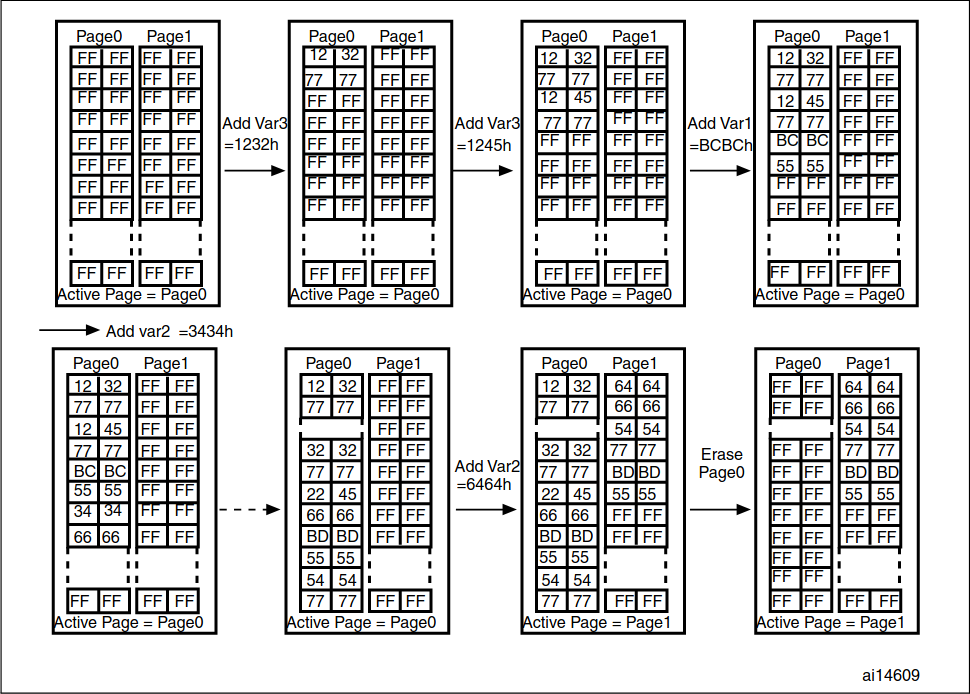
\includegraphics[width=\textwidth]{obrazky/eeprom_emul_principle}
    \caption{EEPROM emulation working principle~\cite{stmicro_an3969_2011}.}
    \label{fig:eeprom_emul}
\end{figure}

Even though the working principle of the EEPROM emulation is simple, there are some technical obstacles in the implementation.
The first obstacle is that the flash memory on the STM32 MCU is split into differently sized sectors and it is required that the sectors have the same size.
Referring to the Reference Manual~\cite{stmicro_stm32f405rg_nodate} there are a some 16~kilobyte sectors that could be used for the emulation, as can be seen in the Figure~\ref{fig:flash_layout}.
Using the 128~kilobyte sectors would also be possible, but given their size copying values from one sector to another would take too much time and also read access times would be higher.

\begin{figure}[H]
    \centering
    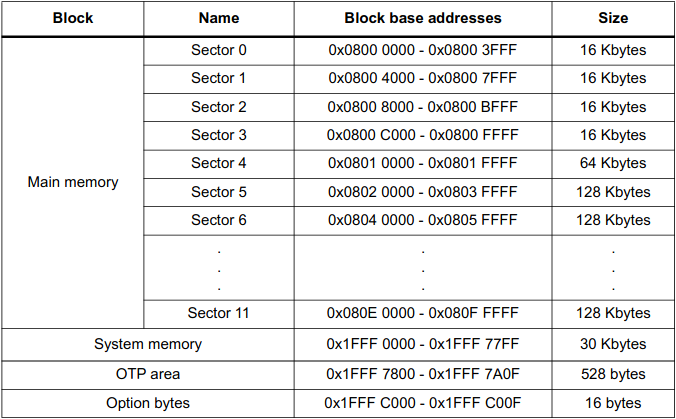
\includegraphics[width=0.8\textwidth]{obrazky/flash_stm}
    \caption{EEPROM emulation working principle~\cite{stmicro_stm32f405rg_nodate}.}
    \label{fig:flash_layout}
\end{figure}

There is however a problem with using the sectors in the beginning of the flash memory as that is where the firmware is usually stored.
The solution to this problem is by leaving the first sector (Sector 0) for the vector table and instructing the linker to place the \textbf{.text} section of the program further in the memory.
According to the documentation of the \textbf{cortex-m} Rust crate~\cite{rust_embedded_wg_rust-embeddedcortex-m-rt_nodate}, this can be achieved by adding the line \textbf{\_stext = ORIGIN(FLASH) + OFFSET} to the linker script, where the \textbf{OFFSET} shall be replaced with the offset of the target sector where we want our program to be stored, in our case \textbf{0x0000C000}, which indicates the start of the Sector 3.

As for the actual implementation of the emulation for the STM32F405, we decided to develop our own, as no suitable Rust crate was available for it.
The development was inspired by a crate that implemented the emulation for STM32F103~\cite{dubrov_idubroveeprom_2020} and by following the implementation in the Application Note.
The functions from flash memory access were adopted from an as of the time of writing unmerged Pull Request into the STM32F4 HAL~\cite{astro_implement_2020}.
An example of accessing the emulated persistent storage can be seen in the following Listing~\ref{lst:eeprom}.

\begin{lstlisting}[caption={An example use of the emulated persistent storage.},label=lst:eeprom]
let mut store = Storage::new(device.FLASH);
store
    .init()
    .expect("Failed to initialize emulated storage.");
store.write_f32(0xbeef, 3.14);
let read = store.read_f32(0xbeef).unwrap();
assert_eq!(read, 3.14);
\end{lstlisting}

As can be seen in the Listing~\ref{lst:eeprom}, first we create the object with a parameter of the flash peripheral, then we initialize the emulated storage - this prepares the sectors that are supposed to be used and then we perform a simple write and read operations on the storage.
